\subsection{Išskirčių tyrimas}
Tyrėme HDI ir vaisinugmo rodiklio išskirtis.
Išskirtis tyrėme pasitelkdami kvartilių metodą. Tai reiškia, kad reikšmę laikėme sąlygine išskirtimi, jei ji prikluasė intervalui $[Q1-3IQR; Q1-1,5IQR) \cup (Q3+1,5IQR; Q3+3IQR]$.

\subsection{Koreliacijos tyrimas}
Pamatavome vaisingumo ir HDI bei vaisingumo ir aukštojo išsilavinimo procento rodiklių koreliacijas. Tai padarėme, pritaikydami Pirsono(angl. Pearson) koreliacijos koeficientą. Jis paskaičiuojamas pagal formulę: 
\begin{equation}
r = \frac{\sum\limits_i (x_i - \bar{x})(y_i - \bar{y})}{\sqrt{\sum\limits_i(x_i - \bar{x})^2}\sqrt{\sum\limits_i(y_i - \bar{y})^2}}
\end{equation}

\begin{table}[h!]
\begin{center}
    \begin{tabular}{|c|c|}
        \hline
        \textbf{Pirsono koreliacijos koeficientas} & \textbf{Reikšmė} \\\hline
        Tarp vaisinigumo ir HDI & -0,819 \\\hline
        Tarp aukštojo išsilavinimo procento ir vaisingumo & -0,399 \\\hline
    \end{tabular}
    \caption{Koreliacijos skaičiavimų rezultatai}
\end{center}
\end{table}

Šių kintamų koreliacijas iliustruoja sklaidos diagramos:
\begin{figure}[h]
    \centering
    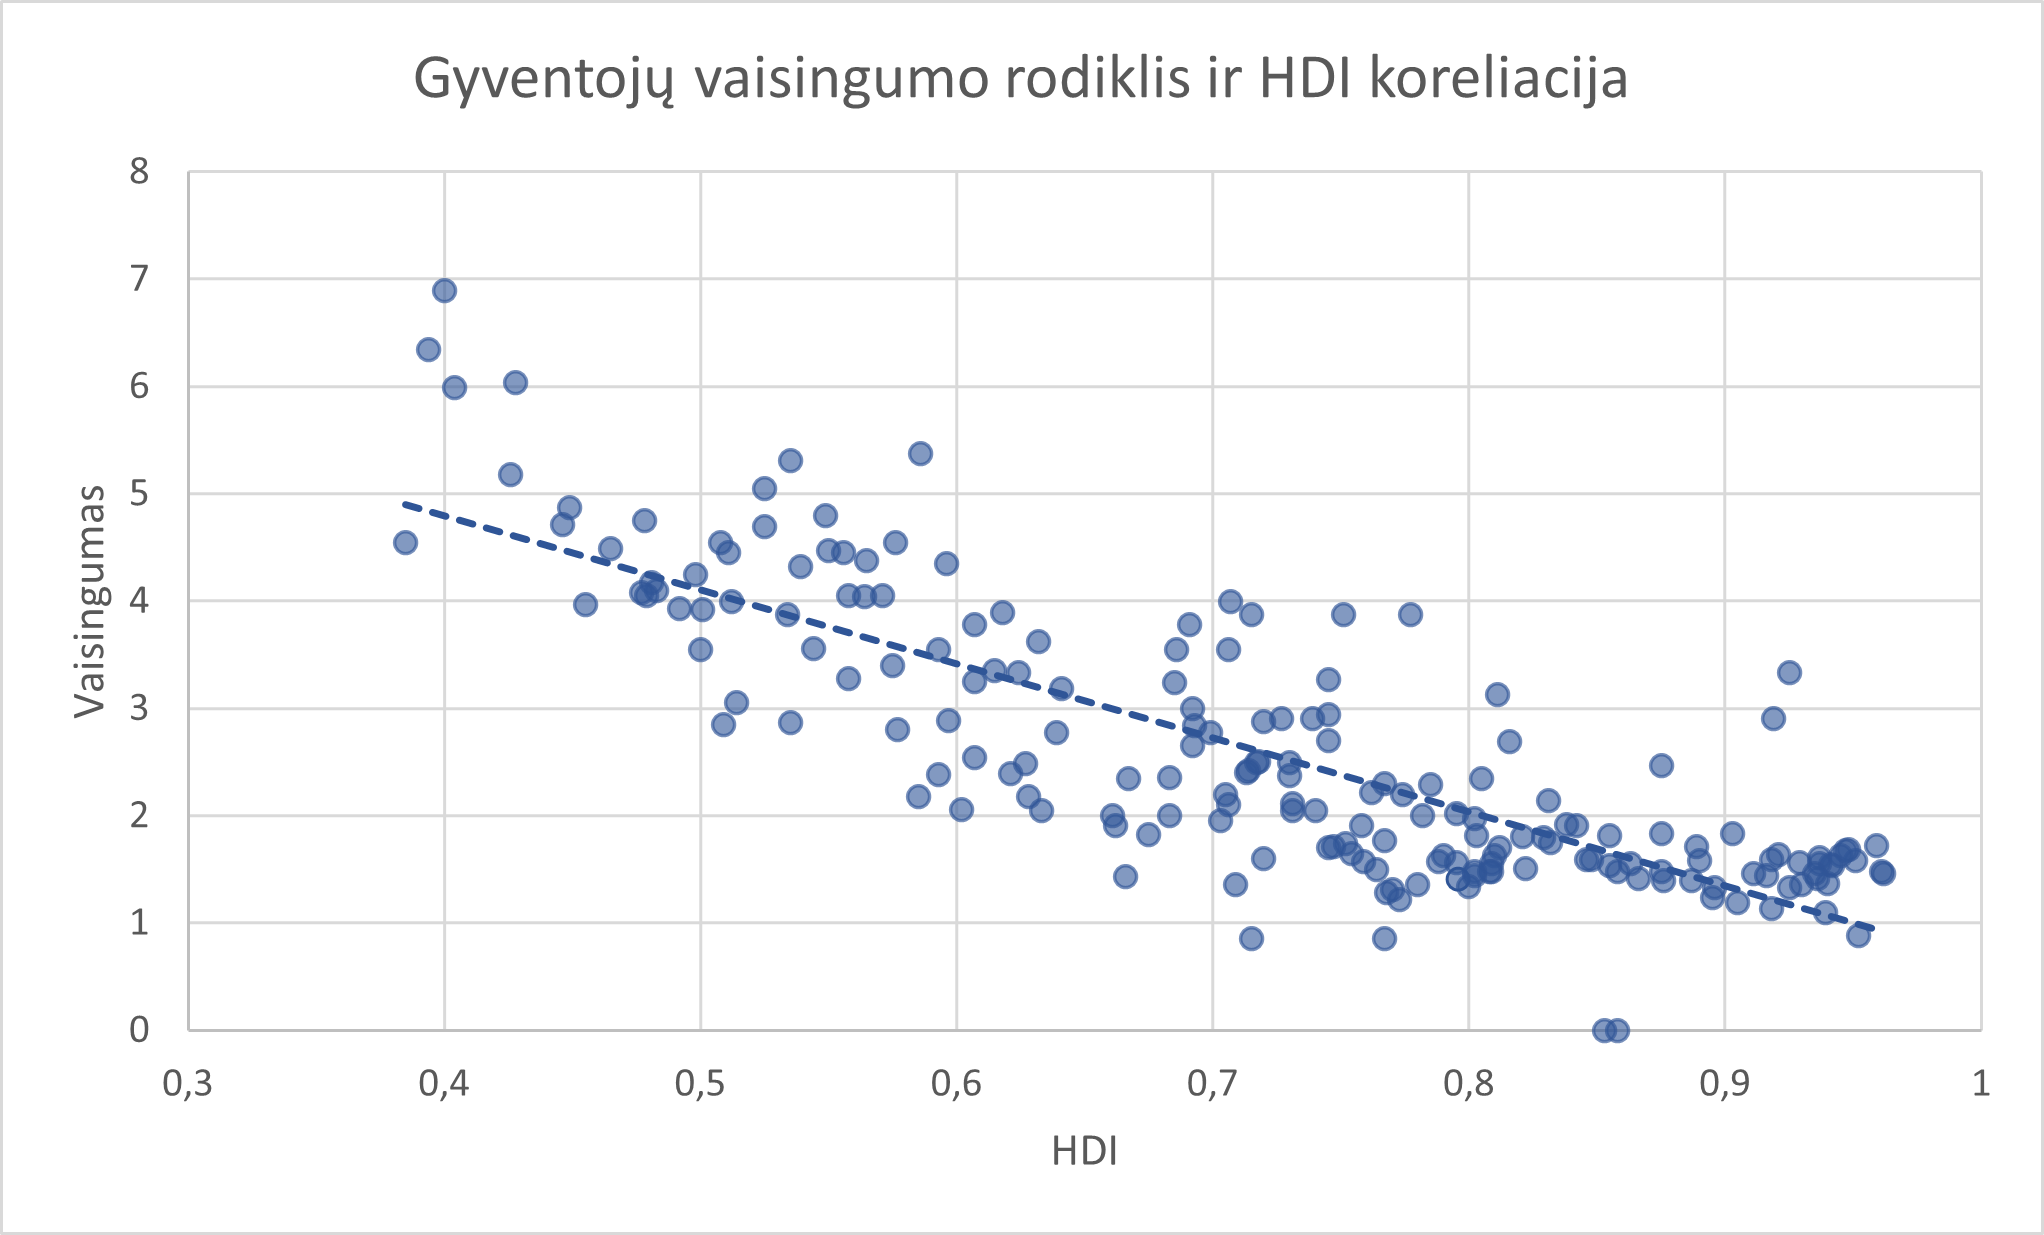
\includegraphics[width=.5\textwidth]{pic/vias_hdi_rod.png}
    \caption{Gyventojų vaisingumo rodiklio ir HDI sklaidos diagrama}
\end{figure}
\begin{figure}[h!]
    \centering
    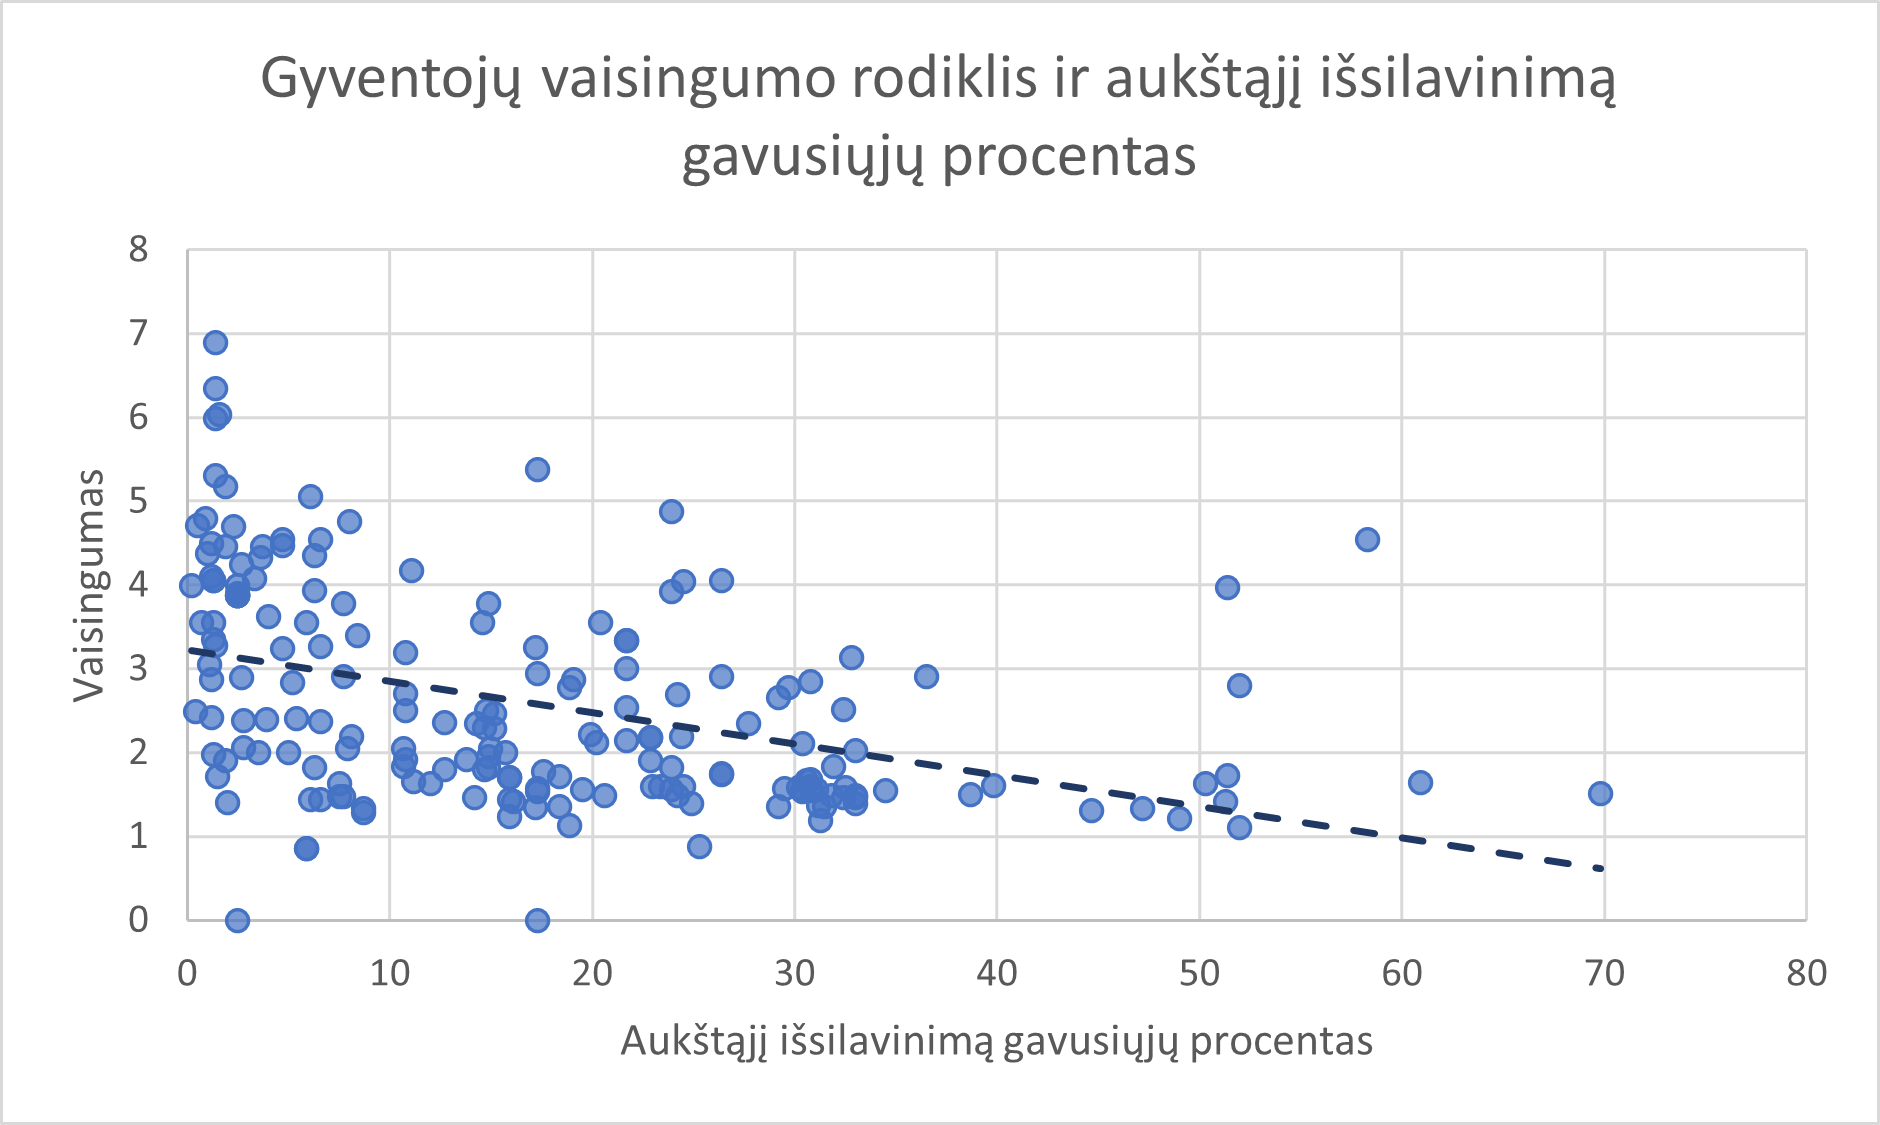
\includegraphics[width=.5\textwidth]{pic/gyv_vais_kor.png}
    \caption{Gyventojų vaisingumo rodiklio ir HDI sklaidos diagrama}
\end{figure}
\subsection{Aukštąjį išsilavinimą gavusiųjų suaugiusiųjų pasiskirtsymo tyrimas} 

Aukštąjį išsilavinimą gavusiųjų suaugiusiųjų pasiskirtsymą iliustruoja histograma:
\begin{figure}[h]
    \centering
    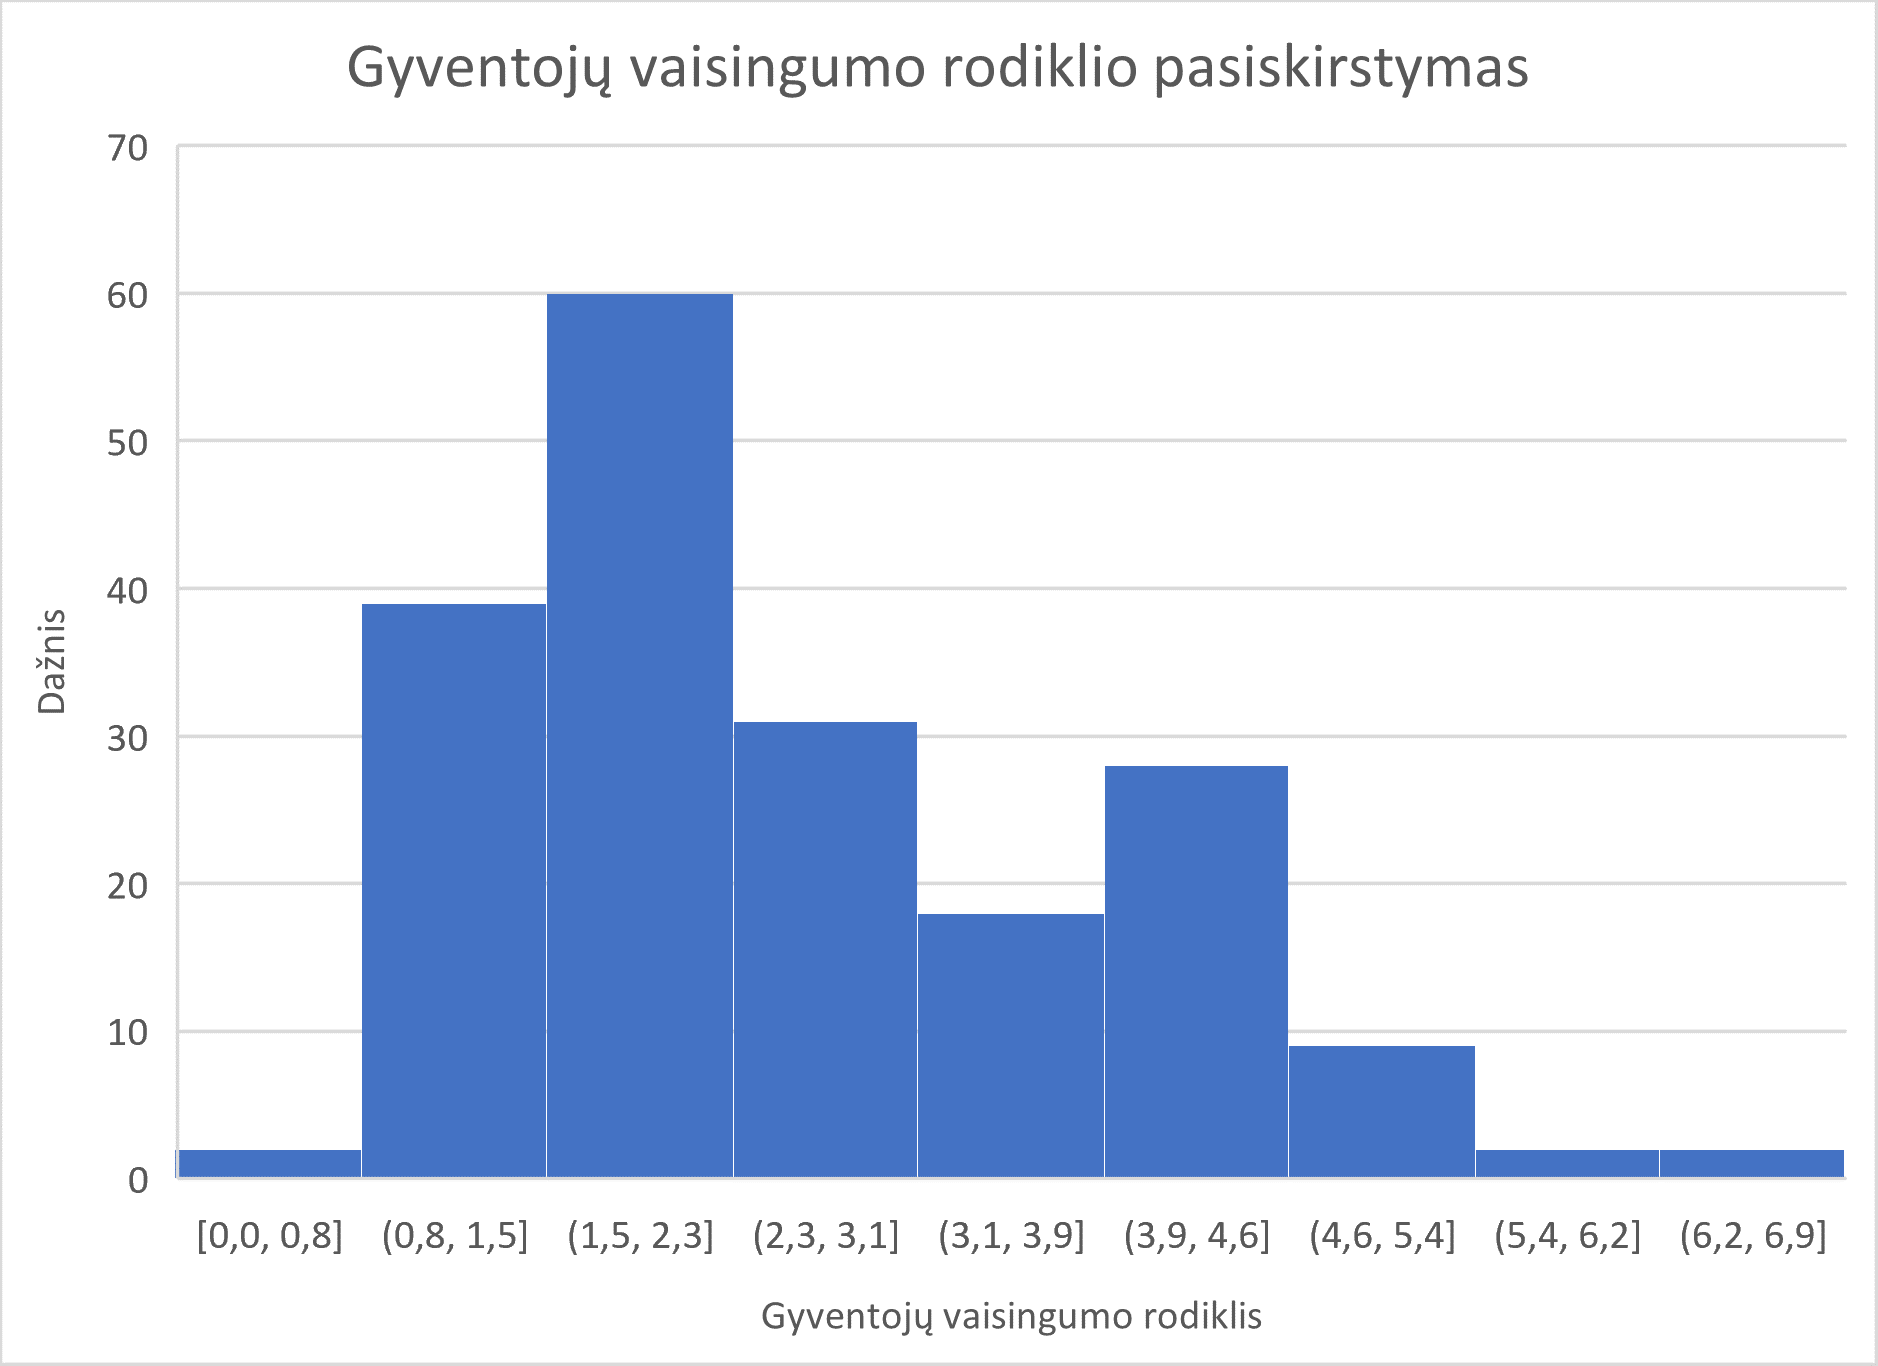
\includegraphics[width=.5\textwidth]{pic/histo.png}
    \caption{Gyventojų vaisingumo rodiklio ir HDI sklaidos diagrama}
\end{figure}

Galima pastebėti, kad skirstinys nėra simetriškas.

\subsection{Vaisingumo pasiskirstymas pasaulyje}
